\subsection{Proceso de extracci\'on}

\noindent
\justify

El concepto de \textit{extracci\'on} se concibe como la obtenci\'on de un producto ``A", procedente de una materia prima ``B", mediante procesos f\'isico-qu\'imicos de separaci\'on de sustancias. La naturaleza de esta materia prima, procesada en la planta de extracci\'on de estudio, es de origen org\'anico; trat\'andose de hojas, ramas, frutos, flores y ra\'ices procedentes de \textbf{plantas arom\'aticas y medicinales}.

%Función de hoja
\newcommand{\hoja}[4]%Cantidad de argumentos
{
	%Contorno
	\draw[pattern=north west lines, pattern color=green!55!black] plot [smooth cycle] coordinates{(#1-#3, #2) (#1 + 0.2*#3, #2 -0.2*#3) (#1 + 2.2*#3, #2 + 1.2*#3) (#1 + 2.9*#3, #2 + 2.7*#3) (#1 + 2.8*#3, #2 + 1.8*#4) (#1 + 2.5*#3, #2 + 2*#4) (#1 + 2.48*#3, #2 + 2.2*#4) (#1 + 2.2*#3, #2 + 2.08*#4) (#1 + 0.7*#3, #2 + 1.9*#4) (#1 - 0.1	*#3, #2 + 3*#3) (#1 - 0.9*#3, #2 + 1.4*#3)};
	\draw[white] plot [smooth cycle] coordinates{(#1-#3, #2) (#1 + 0.2*#3, #2 -0.2*#3) (#1 + 2.2*#3, #2 + 1.2*#3) (#1 + 2.9*#3, #2 + 2.7*#3) (#1 + 2.8*#3, #2 + 1.8*#4) (#1 + 2.5*#3, #2 + 2*#4) (#1 + 2.48*#3, #2 + 2.2*#4) (#1 + 2.2*#3, #2 + 2.08*#4) (#1 + 0.7*#3, #2 + 1.9*#4) (#1 - 0.1	*#3, #2 + 3*#3) (#1 - 0.9*#3, #2 + 1.4*#3)};;
	%Raíz interna
	\draw[white, fill=green!10!white] (#1-1.9*#3, #2-1.5*#3) -- (#1-1.95*#3, #2-1.3*#3) -- (#1-0.2*#3, #2+0.8*#3) -- (#1+0.9*#3, #2+1*#3) -- (#1-0.15*#3, #2+0.9*#3) -- (#1+1.1*#3, #2+2.3*#3) -- (#1+2.1*#3, #2+2.45*#3) -- (#1+1.12*#3, #2+2.4*#3) -- (#1+1.65*#3, #2+3*#3) -- (#1+2.55*#3, #2+3.05*#3) -- (#1+1.7*#3, #2+3.1*#3) -- (#1+2.25*#3, #2+3.7*#3) -- (#1+1.6*#3, #2+3.1*#3) -- (#1+0.7*#3, #2+3.05*#3) -- (#1+1.55*#3, #2+3*#3) -- (#1+0.97*#3, #2+2.4*#3) -- (#1+0.3*#3, #2+2.45*#3) -- (#1+0.9*#3, #2+2.3*#3) -- (#1-0.3*#3, #2+0.9*#3) -- (#1-0.8*#3, #2+1*#3) -- (#1-0.35*#3, #2+0.8*#3) -- (#1-2.1*#3, #2-1.3*#3) -- cycle;
}

\newcommand{\circuloH}[4]
{
	%Círculo
	\hoja{#1}{#2}{#3}{#4};
	\draw[pattern=north west lines, pattern color=green!55!black] (#1 -0.4*#3, #2 + 3*#3) circle (0.9*#3);
	\draw[white] (#1 -0.4*#3, #2 + 3*#3) circle (0.9*#3);
	%Interior
	\draw[white, fill=green!10!white] (#1 - 0.8*#3, #2 + 2.2*#3) -- (#1 +0.2*#3, #2 + 3.65*#3) arc (45:55:0.9*#3) -- (#1 - 0.98*#3, #2 + 2.3*#3) -- cycle;
	%\draw (#1 - 1.08*#3, #2 + 2.4*#3) -- (#1 -0.1*#3, #2 + 3.83*#3);
}

\newcommand{\gota}[4]
{
	\draw[pattern=crosshatch dots, pattern color=blue!30!black] plot [smooth cycle] coordinates{(#1, #2) (#1 + 0.9*#3, #2 + 0.2*#3) (#1 + #3, #2 + #3) (#1, #4) (#1 - #3, #2 + #3) (#1 - 0.9*#3, #2 + 0.2*#3)};
}

\newcommand{\Gota}[4]
{
	\gota{#1}{#2}{#3}{#4};
	\draw[pattern=dots, pattern color=blue!30!white] plot [smooth cycle] coordinates{(#1, #2+0.25*#4) (#1 + 0.45*#3, #2 + 0.2*#3) (#1 + 0.75*#3, #2 + 0.75*#3) (#1, 0.75*#4) (#1 - 0.75*#3, #2 + 0.75*#3) (#1 - 0.45*#3, #2 + 0.2*#3)};
}

\begin{figure}[h!]
	\begin{tikzpicture}
		\circuloH{-4}{0}{0.75}{1.5};
		\node[green!50!black, align=left] at (-5.8,2) {Materia\\ prima};
		\Gota{4}{-0.5}{1.5}{2.75};
		\node[blue!30!black, align=left] at (5.8,2) {Solvente};
		
		%Moléculas
		\draw[fill=red] (-4.7, 2.6) circle (0.08);
		\draw[fill=red] (-4.2, 2.5) circle (0.08);
		\draw[fill=red] (-3.9, 2.2) circle (0.08);
		\draw[fill=red] (-4.3, 2) circle (0.08);
		
		\draw[-triangle 45, fill=black] (-4.5, 3.2) -- (-4.2, 2.5);
		\node[anchor=north, red!50!white] at (-4.5, 3.7) {Producto};
		
		%Flecha solvente
		\coordinate (O) at (4,1);
  		\coordinate (A) at (1,-0.8);

  		\draw (O) to [bend right=15] (A);
  		\draw[-triangle 45, fill=black] (1.01,-0.79) -- (1,-0.8);
  		
  		%Flecha hoja
		\coordinate (OO) at (-3.5,1.5);
  		\coordinate (AA) at (-1,-0.8);

  		\draw (OO) to [bend left=15] (AA);
  		\draw[-triangle 45, fill=black] (-1.01,-0.79) -- (-1,-0.8);

		
		%---Mezcla---
		%vaso
		\draw (-2,-1) -- (-2,-5) -- (-1,-6) -- (1,-6) -- (2,-5) -- (2, -1) -- cycle;
		\node[align=left] at (3.7,-3.2) {Transferencia\\ de masa};
		%Líquido
		\draw[pattern=crosshatch dots, pattern color=blue!30!black] (-1,-6) -- (1,-6) -- (2,-5) -- (2,-3) -- (-2, -3) -- (-2,-5) -- cycle;		
		%Hoja
		\circuloH{-1}{-4.5}{0.25}{0.5}
		\draw[fill=red] (-1.2, -3.7) circle (0.06);
		\draw[fill=red] (-1, -3.75) circle (0.06);
		\draw[fill=red] (-0.7, -4.3) circle (0.06);
		
		\draw[fill=red] (1.2, -4.6) circle (0.06);
		\draw[fill=red] (1.2, -4) circle (0.06);
		
		\draw[white!40!black, -triangle 45, fill=white] (-1, -3.75) -- (1.2, -4);
		\draw[white!40!black, -triangle 45, fill=white] (-0.7, -4.3) -- (1.2, -4.6);
		
		%---Salidas---
		\hoja{-4}{-11}{0.75}{1.5}
		\node[green!50!black, align=left] at (-5.8,-9.5) {Residuo\\ vegetal};
		
		%Flechas
		\coordinate (OOO) at (-0.8,-6.2);
  		\coordinate (AAA) at (-2.1,-7.5);

  		\draw (OOO) to [bend right=15] (AAA);
  		\draw[-triangle 45, fill=black] (-2,-7.3) -- (-2.1,-7.5);
  		
  		\coordinate (OOOO) at (0.8,-6.2);
  		\coordinate (AAAA) at (2.1,-7.5);

  		\draw (OOOO) to [bend left=15] (AAAA);
  		\draw[-triangle 45, fill=black] (2,-7.3) -- (2.1,-7.5);
		
		%Extracto
		\draw[pattern=crosshatch dots, pattern color=blue!30!black] (2,-8) -- (5,-8) -- (5,-11) -- (2,-11) -- cycle;
		\draw[pattern=dots, pattern color=blue!30!white] (2,-8) -- (5,-8) -- (5,-11) -- (2,-11) -- cycle;
		
		\draw[fill=red] (2.5, -8.5) circle (0.08);
		\draw[fill=red] (2.9, -10) circle (0.08);
		\draw[fill=red] (3.5, -9) circle (0.08);
		\draw[fill=red] (4, -10.5) circle (0.08);
		\draw[fill=red] (4.5, -9.5) circle (0.08);
		
		\node[align=left, blue!30!white!50!black] at (6.4,-9.3) {Extracto o\\ aceite esencial};
		
		
	\end{tikzpicture}
	\caption{Extracci\'on.}
	\label{plant_extraction}
\end{figure}

\newpage

\noindent
\justify

El producto obtenido en la extracci\'on puede tratarse de aceite esencial o extracto, dependiendo de las \textit{condiciones termodin\'amicas} del proceso. El aceite esencial se compone de mol\'eculas de bajo y mediano peso molecular y son empleados por las plantas para garantizar su supervivencia. Pertenecen a diferentes clases de sustancias qu\'imicas (fenoles y terpenos, principalmente)$^{\cite{Stashenko2007}}$. Se carcaterizan por un olor t\'ipico y una alta volatilidad. En t\'erminos productivos, se requiere garantizar condiciones de ebullici\'on durante la etapa de transferencia de masa para poder obtener aceite esencial. El solvente (normalmente agua) que est\'a en contacto con la materia prima puede estar en estado l\'iquido (hidrodestilaci\'on)$^{\cite{Pavlic2021}}$ o gaseoso (destilaci\'on por arrastre con vapor)$^{\cite{Balass2013}}$. La mezcla gaseosa entre el vapor del solvente y el aceite esencial es condensada y separada a trav\'es de decantaci\'on.

\noindent
\justify

El \textbf{extracto}, producto de estudio del presente trabajo, se compone de metabolitos y \textit{flavonoides} $\rightarrow$ sustancias de alto peso molecular (no vol\'atiles). Los flavonoides procedentes de algunas especies end\'emicas de la regi\'on (entre ellas, el g\'enero \textit{Lippia}, de la familia Verbenaceae) presentan diferentes propiedades de inter\'es en la medicina tradicional colombiana$^{\cite{Stashenko2013}}$, por lo que representan una interesante oportunidad de innovaci\'on en la elaboraci\'on de productos farmac\'euticos de alto impacto en el mundo$^{\cite{Hennebelle2008}}$, por citar una de sus m\'ultiples aplicaciones. Debido a ello, se han desarrollado estudios referentes a la actividad biol\'ogica de extractos de diferentes especies vegetales (existen m\'as de un mill\'on de art\'iculos cient\'ificos en la base de datos de \textit{science direct} con las palabras clave \textit{natural extracts}); naciendo de all\'i la necesidad de desarrollar plantas de extracci\'on para suplir la demanda en auge de ingredientes naturales. 

\subsection{Objeto de estudio}

\noindent
\justify

Arg\"uello, J.D. \textit{et al} patentaron una planta de extracci\'on para la producci\'on de extractos vegetales$^{\cite{Patente2018}}$. La invenci\'on consiste de un molino de bolas, redise\~nado como recipiente a presi\'on, una unidad evaporadora, un condensador, una torre de enfriamiento, una bomba centr\'ifuga, mecanismo de calentamiento por resistencia el\'ectrica, una bomba de vac\'io, un compresor de aire y un filtro microm\'etrico.

\noindent
\justify

El proceso productivo de la invenci\'on (ver Figura \ref{planta}) consiste en lo siguiente: al material vegetal seco y post-destilado se le realiza un proceso de \textit{molienda} con la ayuda de un agente dispersante (material abrasivo, normalmente arena de r\'io), disminuyendo el tama\~no de part\'icula del material vegetal. A esta mezcla s\'olida entre el material vegetal pulverizado y la arena de r\'io se eluye un solvente, produci\'endose el fen\'omeno de extracci\'on mostrado en la Figura \ref{plant_extraction} y dando paso a la etapa de \textbf{eluci\'on y filtrado}. El molino de bolas se adapta, con la ayuda de un mecanismo rotatorio, para dar paso a la separaci\'on de la mezcla heterog\'enea s\'olido - l\'iquida. La mezcla se presuriza con la ayuda del compresor de aire y esta se separa a trav\'es del filtro microm\'etrico en las fases s\'olida y l\'iquida de la mezcla. La fase l\'iquida consiste en la mezcla homog\'enea entre el solvente y el extracto. Finalmente, se emplea un sistema de evaporaci\'on al vac\'io para separar el solvente del extracto (producto final). 

\begin{figure}[h!]
	\centering
	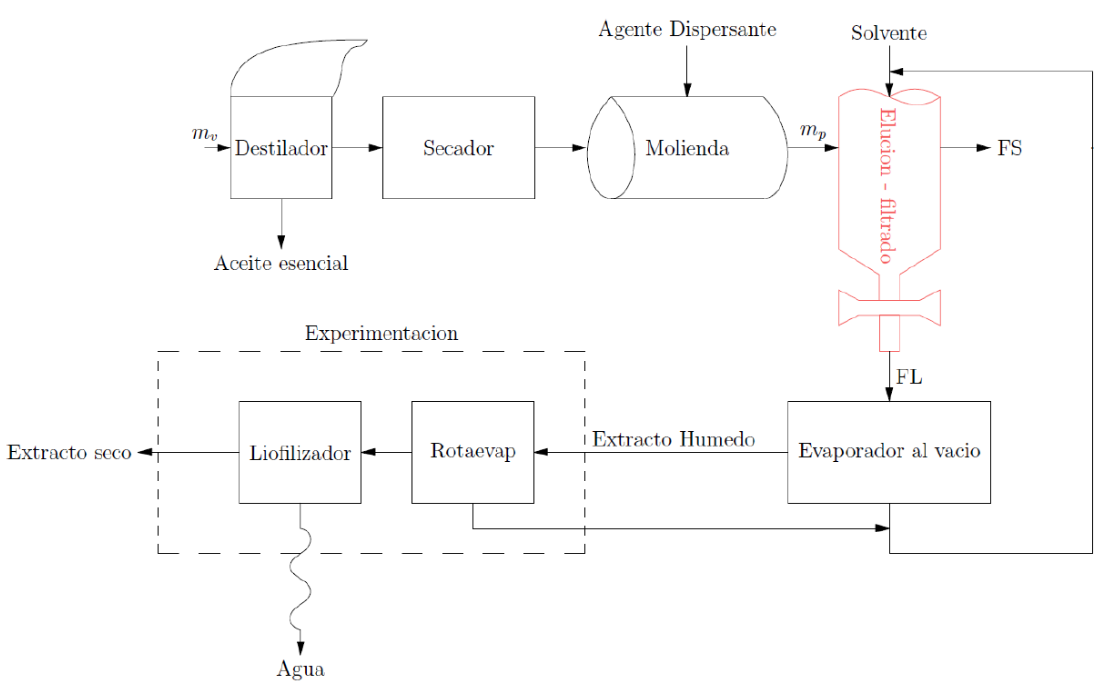
\includegraphics[width=\textwidth]{Images/Planta.png}
	\caption{Proceso productivo de la planta de extracci\'on.}
	\label{planta}
\end{figure}

\noindent
\justify

De la Figura \ref{planta}: $m_v$ es la materia prima vegetal, el agente dispersante se trata de un material auxiliar altamente abrasivo (en la mayor\'ia de aplicaciones, se trata de arena de r\'io), $m_p$ es la mezcla entre material vegetal pulverizado y el agente dispersante, $FS$ se trata del residuo s\'olido y $FL$ es la fase l\'iquida $\rightarrow$ mezcla homog\'enea entre el solvente y el extracto.

\noindent
\justify

En pruebas experimentales desarrolladas a la planta construida, se identific\'o que la etapa de eluci\'on y filtrado es el \textit{cuello de botella} del proceso productivo; debido a que el tiempo de esta etapa es cerca del doble del tiempo requerido por las otras etapas. Por esta raz\'on, en este trabajo se eval\'ua la viabilidad de un sistema de sedimentaci\'on de placas paralelas como sistema de eluci\'on y filtrado de la planta de extracci\'on; desarrollando, adem\'as, una metodolog\'ia de dise\~no autom\'atico a trav\'es de herramientas de c\'odigo abierto. Esta metodolog\'ia automatiza el proceso de dise\~no empleando m\'etodos num\'ericos (cap\'itulo \ref{CFD-DEM}) que permiten predecir el comportamiento fluido-part\'icula durante la separaci\'on de las fases s\'olida y l\'iquida. La metodolog\'ia fue validada mediante un estudio experimental reportado en la literatura (cap\'itulo \ref{validacion}). 


\newpage

\subsection{Organizaci\'on de la tesis}

\noindent
\justify

El presente trabajo se organiza de la siguiente manera:

\begin{table}[h!]
	\centering
	\begin{tabular}{|c|c|p{6cm}|}
		\hline
		\begin{tabular}[c]{@{}l@{}}\textbf{N\'umero} \\ \textbf{del cap\'itulo}\end{tabular} & \textbf{Nombre del cap\'itulo} & \textbf{Objetivo} \\ \hline
		- & Introducci\'on & Explica brevemente el caso de estudio y la raz\'on por la que se desarroll\'o el presente trabajo. \\ \hline
		1 & Marco te\'orico & Contiene todos los conceptos y teor\'ias empleadas para la ejecuci\'on de la tesis. \\ \hline
		2 & Metodolog\'ia & Explica de forma detallada la l\'ogica de ejecuci\'on. \\ \hline
		3 & Resultados & Contiene todos los resultados obtenidos del trabajo de investigaci\'on \\ \hline
		4 & An\'alisis de resultados & Expone el an\'alisis de los resultados obtenidos. \\ \hline
		5 & Validaci\'on del modelo & Resuelve, mediante el m\'etodo CFD-DEM, un caso experimental reportado en la literatura. \\ \hline
		- & Conclusiones & Expone las conclusiones alcanzadas con base en los resultados obtenidos y al an\'alisis desarrollado. \\ \hline
		- & Recomendaciones & Cap\'itulo en donde se explican los retos y avances que complementan la presente investigaci\'on. \\ \hline
		- & Anexo A & Contiene evidencia visual de la funcionalidad del software desarrollado con herramientas de c\'odigo abierto. \\ \hline
	\end{tabular}
	\caption{Organizaci\'on de la tesis.}
	\label{organi}
\end{table}